\documentclass[12pt, a4paper]{article}
% \usepackage{ctex}
\usepackage[margin=1in]{geometry} 
\usepackage{amsmath,amsthm,amssymb}
\usepackage{bm}
\usepackage{cases}
\usepackage{graphicx}
\usepackage{hyperref}
\hypersetup{hidelinks}
\usepackage{amsfonts}
\usepackage{authblk}
\title{PRML Note\\C01 Introduction}
\author{Yang Zhao}
\affil{Department of Automation, Tsinghua University}
\date{}

\begin{document}
    \maketitle
    \begin{itemize}
        \item Generalization is a central goal in PR
        \item The Original input variables are typically
        preprocessed. The Test data must be preprocessed
        using the same steps as training data.
        \item  $\text{feature extraction}
        \begin{cases}
        &\text{PR problem easy to solve}\\
        &\text{speed up computation}
        \end{cases}$
        \item  $\text{supervised learning}
        \begin{cases}
        &\text{classification}\\
        &\text{regression}
        \end{cases}$\\
        $\text{unsupervised learning}
        \begin{cases}
        &\text{clustring}\\
        &\text{density estimation}\\
        &\text{dimensions reduction}
        \end{cases}$
    \end{itemize}
    \section{Example: Polynomial Curve Fitting}
    \begin{itemize}
        \item Linear Model:
        \begin{equation}\label{equ:square}
            y(x,\bm{w})=w_0+w_1x+w_2x^2+\cdots+w_Mx^M=\sum_{j=0}^Mw_jx^j
        \end{equation}
        $\bm{w}$ determined by 
        \[
            argmin_{\bm{w}^*}E(\bm{w})=\frac{1}{2}\sum_{n=1}^N
            \{y(x_n,\bm{w})-t_n\}^2
        \]
        which is called error funtion\\
        $M$: model comparison or model selection\\
        \[
            E_{RMS}=\sqrt{\frac{2E(\bm{w}^*)}{N}}
            \]
        in which the division by $N$ allows us to compare different
        size of data sets.
        \begin{figure}[ht]
            \begin{center}
                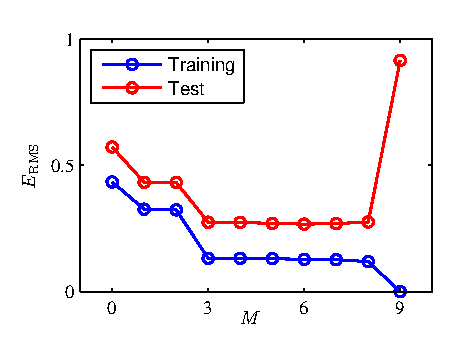
\includegraphics[width=3in]{figures/Figure1_5.eps}
                \caption{Graphs of the RMS error evalutated on the training 
                set and on an independent test set for various values of M}
            \end{center}
        \end{figure}
        \item Large value of M $\rightarrow$ Polynomials 
        flexible $\rightarrow$ increasing tuned to the random
        noises on target values
        \item The larger the data set, the more complex the model that
        we can afford to fit
        \item By adopting a Bayesian approach, over-fitting can be avoided.\\
        In a Bayesian model, the effective number of parameters adapts
        automatically to the size of the data set
        \item regularization:
        \[
            \widetilde{E}(\bm{w})=\frac{1}{2}\sum_{n=1}^N\{y(x_n,\bm(w))
            -t_n\}^2+\frac{\lambda}{2}\Vert\bm{w}\Vert^2
            \]
        \begin{enumerate}
            \item shrinkage in statistics
            \item ridge regression
            \item weight decay in NN
        \end{enumerate}
        \begin{figure}[ht]
            \begin{center}
                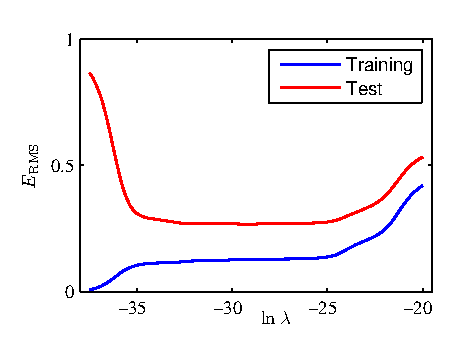
\includegraphics[width=3in]{figures/Figure1_8.eps}
                \caption{Graphs of the RMS error evalutated on the training 
                set and on an independent test set for $ln\lambda$}
            \end{center}
        \end{figure}
        \item $\Vert\bm{w}\Vert^2=\bm{w}^T\bm{w}=w_0^2+w_1^2+\cdots+w_M^2$
        \begin{enumerate}
            \item $w_0^2$ is often omitted. if not, the result will depend
            on the choice of the origin for the target variable
            \item $\frac{\lambda_1}{2}w_0^2+\frac{\lambda_2}{2}(w_1^2+
            \cdots+w_M^2)$ is also OK 
        \end{enumerate}
        \item $\text{data set}\begin{cases}
            &\text{training set}\rightarrow\bm{w}\\
            &\text{validation set(hold-out set)}\\
            &\rightarrow M,\lambda
            \text{ which is too wasteful of data set}\\
            &\text{test set}
            \end{cases}$
    \end{itemize}
    \section{Probability Theory}
    \begin{itemize}
        \item the rules of Probability
        \begin{enumerate}
            \item sum rule: $P(x)=\sum_YP(x,Y)$
            \item product rule: $P(x,Y)=P(Y|x)P(x)$\\
            in which $P(x)$ is called marginal probability and $P(Y|x)$ is 
            called conditional probability.
        \end{enumerate}
        \item Bayes' Theorem:
        \[
            P(Y|X)=\frac{P(X|Y)P(Y)}{P(X)}=\frac{P(X|Y)P(Y)}{\sum_Y{P(X|Y)P(Y)}}
            \]
        \item a nonlinear change of variable $x=g(y)$\\
        consider a probability density $p_x(x)$ that correspond to a density $p_y(y)$.
        Observations falling in the range $(x,x+\delta x)$ will be transformed into the
        range $(y, y+\delta y)$ where $p_x(x)\simeq p_y(y)$
        \[
            p_y(y)=p_x(x)\Big\vert\frac{dx}{dy}\Big\vert=p_x(g(y))\vert g'(y)\vert
            \]
        So, the concept of the max of a probability density is dependent on the choice
        of variable.
        \item Expectations: $\mathbb{E}[f]=\sum_xp(x)f(x)\simeq \frac{1}{N}\sum_{n=1}
        ^{N}f(x_n)$\\
        Conditional Expectations: $\mathbb{E}[f|y]=\sum_xp(x|y)f(x)$
        \item Variances: \[Var[f]=\mathbb{E}\{(f(x)-\mathbb{E}[f(x)])^2\}=
        \mathbb{E}\{f^2(x)\}-\mathbb{E}^2\{f(x)\}\]
        Corvariances: \[cov(x,y)=\mathbb{E}_{x,y}\lbrack\{x-\mathbb{E}\lbrack x\rbrack\}
        \{y-\mathbb{E}\lbrack y\rbrack\}\rbrack=\mathbb{E}_{xy}\lbrace xy\rbrace-
        \mathbb{E}\lbrace x\rbrace\mathbb{E}\lbrace y\rbrace\]
        \item a prior probability distribution $p(\bm{w})$\\
        Observed data $D=\{t_1,t_2,\cdots,t_N\}$ is expressed through the conditional
        probability $p(D|\bm{w})$
        \[
            p(\bm{w}|D)=\frac{p(D|\bm{w})P(\bm{w})}{p(D)}
            \]
        in which $p(D|\bm{w})$ is called likelihood function which expresses how 
        probable the observed data set is for different settings of the parameters $\bm{w}$
        and $p(D)$ is called normalization constant which is 
        $p(D)=\int p(D|\bm{w})p(\bm{w})d\bm{w}$
        \item A data set of observations $X=(x_1,x_2,\cdots,x_N)^T$,i,i,d, the likelihood
        function is
        \[
            p(X|\mu,\sigma^2)=\prod_{n=1}^N\mathcal{N}(x_n|\mu,\sigma^2)
            \]
        and the log likelihood function can be written in the form
        \[
            lnp(x|\mu,\sigma^2)=-\frac{1}{2\sigma^2}\sum_{n=1}^N(x_n-\mu)^2-\frac{N}{2}
            ln(\sigma^2)-\frac{N}{2}ln(2\pi)
            \]
        \item find the $\mu$ and $\sigma^2$ to max this likelihood function and the maximum
        likelihood solution is\\
        $ \begin{cases}
        &\mu_{ML}=\frac{1}{N}\sum_{n=1}^Nx_n\\
        &\sigma_{ML}^2=\frac{1}{N}\sum_{n=1}^{N}(x_n-\mu_{ML})^2
        \end{cases}$\\
        and the expectation of it is\\
        $\begin{cases}
        &\mathbb{E}\lbrace \mu_{ML}\rbrace=\mu\\
        &\mathbb{E}\lbrace \sigma_{ML}^2\rbrace=(\frac{N-1}{N})\sigma^2
        \end{cases}$\\
        so
        \[\widetilde{\sigma}^2=\frac{N}{N-1}\sigma_{ML}^2=\frac{1}{N-1}
        \sum_{n=1}^N(x_n-\mu_{ML})^2\]
        \item bootstrap: suppose data set consists of $N$ data points $\bm{X}=\{\bm{x}_1,
        \cdots,\bm{x}_N\}$, we can drawing $N$ data points at random from $\bm{X}$ to create 
        a new data set $\bm{X}_B$. This process can be repeated $L$ times
        \item maximum posterior(MAP): suppose training data comprising $N$ input values 
        $\bm{x}=(x_1,x_2,\cdots,x_N)^T$ and their corresponding target values $\bm{t}=(t_1,
        t_2,\cdots,t_N)^T$. We have
        \begin{equation}
            p(t|x,\bm{w},\beta)=\mathcal{N}(t|y(x,\bm{w}),\beta^{-1})
        \end{equation}
        where $y(x,\bm{w})$ is given by equation (\ref{equ:square}). So the likelihood function is
        given by
        \[
            p(\bm{t}|\bm{x},\bm{w},\beta)=\prod_{n=1}^N\mathcal{N}(t_n|y(x_n,\bm{w}),\beta^{-1})
            \]
        and the log likelihood function is 
        \[
            lnp(\bm{t}|\bm{x},\bm{w},\beta)=-\frac{\beta}{2}\sum_{n=1}^N\{y(x_n,\bm{w})-t_n\}^2
            +\frac{N}{2}ln\beta-\frac{N}{2}ln2\pi
            \]
        If we consider a prior distribution over $\bm{w}$,
        \[
            p(\bm{w}|\alpha)=\mathcal{N}(\bm{w}|\bm{0},\alpha^{-1}\bm{I})
            \]
        then the posterior distribution for $\bm{w}$ is 
        \[
            p(\bm{w}|\bm{x},\bm{t},\alpha,\beta)\propto p(\bm{t}|\bm{x},\bm{w},\beta)p(\bm{w}|\alpha)
            \]
        and we should maximize the log posterior function
        \[
            \frac{\beta}{2}\sum_{n=1}^N\{y(x_n,\bm{w})-t_n\}^2+\frac{\alpha}{2}\bm{w}^T\bm{w}
            \]
        \item Bayesian curve fitting: Given training data $\bm{x}$ and $\bm{t}$, along with a new
        point $x$, we want to predict the value of $t$, 
        \[
            p(t|x,\bm{x},\bm{t})=\int p(t|x,\bm{w})p(\bm{w}|\bm{x},\bm{t})d\bm{w}
            \]
    \end{itemize}
    \section{Model Selection}
    \begin{itemize}
        \item data is plentiful: train a range of models or a model with a range of values for its
        complexity params.
        \item  data is limited: cross-validation
        \item An ideal approach: 
        \begin{enumerate}
            \item only rely on the training data
            \item allow multiple hyperparameters and model types to be compared in a single 
            training run
        \end{enumerate}
        therefore, find a measure of performance which depends only on the training data, not
        suffer from bias to over-fitting.
    \end{itemize}
    \section{The Curse of Dimensionality}
    \begin{itemize}
        \item Not all intuitions developed in spaces of low dimensionality will generalize to 
        spaces of many dimensions
        \item real data 
        \begin{enumerate}
            \item often be confined in lower effective dimensionality
            \item exhibit smooth properties
        \end{enumerate}
    \end{itemize}
    \section{Decision Theory}
    \begin{itemize}
        \item For 2-classes, minimize
        \begin{align*}
            p(mistake)&=p(x\in R_1,C_2)+p(x\in R_2, C_1)\\
            &=\int_{R_1}p(x,C_2)dx+\int_{R_2}p(x,C_1)dx
        \end{align*}
        if $p(x,C_1)>p(x,C_2)$, which is the same as $p(C_1|x)p(x)>p(C_2|x)p(x)$ i.e. 
        $p(C_1|x)>p(C_2|x)$, $x\rightarrow C_1$
        \begin{figure}[ht]
            \begin{center}
                \includegraphics[width=0.6\textwidth]{figures/Figure1_24.eps}
                \caption{The joint probability of two classes}
            \end{center}
        \end{figure}
        \item For $k$-classes, maximize
        \begin{align*}
            p(correct)&=\sum_{k=1}^K\int_{R_k}p(x,C_k)dx\\
            &=\sum_{k=1}^K\int_{R_k}p(C_k|x)p(x)dx
        \end{align*}
        find the max $p(C_k|x)$ and $x\rightarrow C_k$
        \item reject option: if $p(C_k|x)<\theta$, do not classify $x$
        \begin{enumerate}
            \item $\theta=1$, reject all samples
            \item For $k$-classes, $\theta<\frac{1}{k}$, No sample is rejected
        \end{enumerate}
        \item Generative model: find the joint distribution $p(C_k,x)$ and then find
        the posterior distribution $p(C_k|x)$ to make decision using decision theory. 
        This can be used to detect new data point with low probability, which is known
        as outlier detection or novelty detection.
        \item Discriminative model: find the posterior distribution directly, and use 
        it to make decision.
        \item Discriminant function: only a function, the input is $x$ and the output is
        the class label.
        \item Compensating for class prior: In training data $n(C_1)=a$ and $n(C_2)=b$, if 
        $a\gg b$ ,it is not likely to generalize well. From the training data we can get a 
        balanced data set. From the balanced data we can get the posterior $p(C_1|x)$ and 
        $p(C_2|x)$. And the goal data set we want to apply to is $n(C_1)=a'$ and $n(C_2)=b'$, 
        so the posterior we use is \[\widetilde{p}(C_1|x)=\frac{p(C_1|x)}{\frac{a}{a+b}}
        \frac{a'}{a'+b'}\] and \[\widetilde{p}(C_2|x)=\frac{p(C_2|x)}{\frac{b}{a+b}}
        \frac{b'}{a'+b'}\] then normalize to ensure
         \[\widetilde{p}(C_1|x)+\widetilde{p}(C_2|x)=1\]
         Explaination: 
         \[\frac{p(C_1|x)}{\frac{a}{a+b}}\propto \text{likelihood function}=p(x|C_1)\]
         \item Combining models: $p(\bm{x_I},\bm{x_B}|C_k)=p(\bm{x_I}|C_k)p(\bm{x_B}|C_k)$,
        so we can get
        \begin{align*}
            p(C_k|\bm{x_I},\bm{x_B})&\propto p(\bm{x_I},\bm{x_B}|C_k)p(C_k)\\
            &\propto p(\bm{x_I}|C_k)p(\bm{x_B}|C_k)p(C_k)\\
            &\propto \frac{p(C_k|\bm{x_I})p(C_k|\bm{x_B})}{p(C_k)}
        \end{align*}
        \item Calculus of Variations: if $J(y)=\int_{x_1}^{x_2}\mathcal{L}(x,y(x),y'(x))dx$, 
        we have 
        \begin{equation}
            \label{CalculusVariations}
            \frac{\partial J(y)}{\partial y}=\frac{\partial\mathcal{L}}{\partial f}-\frac{d}{dx}
            \frac{\partial\mathcal{L}}{\partial f'}
        \end{equation}
        which is called Euler-Lagrange Equation.
        \item Incuring a Loss function $\mathcal{L}(t,y(\bm{x}))$, the average, or expected, 
        loss is given by
        \begin{equation}
            \label{equ:loss:expectation}
            \mathbb{E}\lbrack L\rbrack=\iint\mathcal{L}(t,y(\bm{x}))p(\bm{x},t)d\bm{x}dt
        \end{equation}
        A common choice of loss funtion is $\mathcal{L}(t,y(\bm{x}))=\{y(\bm{x}-t)\}^2$, 
        using the Calculus of Variations
        \[
            \frac{\partial\mathbb{E}\lbrack L\rbrack}{\partial y(\bm{x})}=
            2\int\{y(\bm{x})-t\}p(\bm{x},t)dt=0
            \]
        So we have
        \[
            y(\bm{x})=\frac{\int tp(\bm{x},t)dt}{p(\bm{x})}\int tp(t|\bm{x})dt=
            \mathbb{E}_t\lbrack t|\bm{x}\rbrack
            \]
        \item from equation (\ref{equ:loss:expectation}), we can rewrite to
        \begin{align}
            \mathbb{E}\lbrack L\rbrack&=\iint\{y(\bm{x}-\mathbb{E}\lbrack t|\bm{x}\rbrack
            +\mathbb{E}\lbrack t|\bm{x}\rbrack-t)\}^2p(\bm{x},t)d\bm{x}dt\nonumber\\
            \label{equ:loss:expectation2}
            &=\int\{y(\bm{x})-\mathbb{E}\lbrack t|\bm{x}\rbrack\}^2p(\bm{x})d\bm{x}+
            \int Var\lbrack t|\bm{x}\rbrack p(\bm{x})d\bm{x}
        \end{align}
        The process to get the equation (\ref{equ:loss:expectation2}) is below:
        \begin{enumerate}
            \item $\{y(\bm{x}-t)\}^2=\{y(\bm{x})-\mathbb{E}\lbrack t|\bm{x}\rbrack\}^2
            +2\{y(\bm{x})-\mathbb{E}\lbrack t|\bm{x}\rbrack\}\{\mathbb{E}\lbrack t|\bm{x}
            \rbrack-t\}+\{\mathbb{E}\lbrack t|\bm{x}\rbrack-t\}^2$
            \item $p(\bm{x},t)=p(t|\bm{x})p(\bm{x})$
            \item \begin{align*}
            \mathbb{E}\lbrack L\rbrack_1&=\iint\{y(\bm{x})-\mathbb{E}\lbrack t|\bm{x}
            \rbrack\}^2p(\bm{x},t)d\bm{x}dt\\
            &=\iint\{y(\bm{x})-\mathbb{E}\lbrack t|\bm{x}\rbrack\}^2p(t|\bm{x})p(\bm{x})d\bm{x}dt\\
            &=\int\{y(\bm{x})-\mathbb{E}\lbrack t|\bm{x}\rbrack\}^2p(\bm{x})
            (\int p(t|\bm{x})dt)d\bm{x}\\
            &=\int\{y(\bm{x})-\mathbb{E}\lbrack t|\bm{x}\rbrack\}^2p(\bm{x})d\bm{x}
            \end{align*}
            \item \begin{align*}
                \mathbb{E}\lbrack L\rbrack_2&=\iint\{y(\bm{x})-\mathbb{E}\lbrack t|\bm{x}\rbrack\}
                \{\mathbb{E}\lbrack t|\bm{x}\rbrack-t\}p(t|\bm{x})p(\bm{x})d\bm{x}dt\\
                &=\int\{y(\bm{x})-\mathbb{E}\lbrack t|\bm{x}\rbrack\}p(\bm{x})
                (\int\{\mathbb{E}\lbrack t|\bm{x}\rbrack-t\}p(t|\bm{x})dt)d\bm{x}\\
                &=\int\{y(\bm{x})-\mathbb{E}\lbrack t|\bm{x}\rbrack\}p(\bm{x})
                (\mathbb{E}\lbrack t|\bm{x}\rbrack-\int tp(t|\bm{x})dt)d\bm{x}\\
                &=\int\{y(\bm{x})-\mathbb{E}\lbrack t|\bm{x}\rbrack\}p(\bm{x})
                (\mathbb{E}\lbrack t|\bm{x}\rbrack-\mathbb{E}\lbrack t|\bm{x}\rbrack)d\bm{x}\\
                &=0
            \end{align*}
            \item \begin{align*}
                \mathbb{E}\lbrack L\rbrack_3&=\iint\{\mathbb{E}\lbrack t|\bm{x}\rbrack-t\}^2
                p(t|\bm{x})p(\bm{x})d\bm{x}dt\\
                &=\iint\{\mathbb{E}^2\lbrack t|\bm{x}\rbrack-2t\mathbb{E}\lbrack t|\bm{x}
                \rbrack+t^2\}p(t|\bm{x})p(\bm{x})d\bm{x}dt\\
                &=\int\{-\mathbb{E}^2\lbrack t|\bm{x}\rbrack+\mathbb{E}\lbrack t^2|\bm{x}\rbrack\}
                p(\bm{x})d\bm{x}\\
                &=\int Var\lbrack t|\bm{x}\rbrack p(\bm{x})d\bm{x}
            \end{align*}
            \item $\mathbb{E}\lbrack L\rbrack=\mathbb{E}\lbrack L\rbrack_1+\mathbb{E}\lbrack 
            L\rbrack_2+\mathbb{E}\lbrack L\rbrack_3$
        \end{enumerate}
        \item Squared loss can lead to very poor results.
        \item The Minkowski loss $\vert y(\bm{x})-t\vert^q$
    \end{itemize}
    \section{Information Theory}
    \begin{itemize}
        \item $h(x)=-log_2p(x)$
        \item the entropy of the random variable $x$(bit): $H\lbrack x\rbrack=-\sum_xp(x)log_2p(x)$ 
        and the entropy of the random variable $x$(nat): $H\lbrack x\rbrack=-\frac{1}{ln2}\sum_xp(x)lnp(x)$
        \item if $p(x)=0$, we have $p(x)log_2p(x)=0$
        \item The conditional entropy of $y$ given $x$: 
        \[
            H\lbrack y|x\rbrack=-\iint p(y,x)lnp(y|x)dydx    
        \]
        and $H\lbrack x,y\rbrack=H\lbrack y|x\rbrack+H\lbrack x\rbrack$
        \item relative entropy or KL divergence between the distribution $p(x)$ and $q(x)$
        \begin{align}
            KL(p\Vert q)&=-\int p(x)lnq(x)dx-(-\int p(x)lnp(x)dx)\nonumber\\
            &=-\int p(x)ln\Big\{\frac{q(x)}{p(x)}\Big\}dx
        \end{align}
        Note that $KL(p\Vert q)\neq KL(q\Vert p)$ and $KL(p\Vert q)\geq 0$ with equality, if and only if 
        $p(x)=q(x)$
        \item the mutual information between the variables $x$ and $y$
        \begin{align}
            I\lbrack x,y\rbrack&=KL(p(x,y)\Vert p(x)p(y))\nonumber\\
            &=-\iint p(x,y)ln\Big\{\frac{p(x)p(y)}{p(x,y)}\Big\}dxdy
        \end{align}
        Note that $I\lbrack x,y\rbrack\geq 0$ with equality, if and only if $x$ and $y$ are independent
        and we have $I\lbrack x,y\rbrack=H\lbrack x\rbrack-H\lbrack x|y\rbrack
        =\lbrack y\rbrack-H\lbrack y|x\rbrack$
    \end{itemize}
    \section{Appendix}
    \begin{itemize}
        \item To get the Euler-Lagrange equation\ref{CalculusVariations}, consider the function
        \begin{equation*}
            J(y)=\int_{x_1}^{x_2}L(x,y(x),y'(x))dx
        \end{equation*}
        where
        $x_1,x_2$ are constants, $y(x)$ is twice continuously differentiable, $y'(x)=dy/dx$, 
        $L(x,y(x),y'(x))$ is twice continuously differentiable with respect to its arguments $x,y,y'$.
        If the funtion $J(y)$ attains a local minimum at $f$, and $\eta$ is an arbitrary function 
        that has at least one derivative and vanishes at the endpoints $x_1$ and $x_2$, then for any 
        number $\epsilon$ close to 0,
        \begin{equation*}
            J(f)\le J(f+\epsilon\eta)
        \end{equation*}
        Let $\Phi(\epsilon)=J(f+\epsilon\eta)$, and the function $\Phi(\epsilon)$ has a minimum at
        $\epsilon=0$, thus
        \begin{equation*}
            \Phi'(0)=\frac{d\Phi}{d\epsilon}\Big\vert_{\epsilon=0}=\int_{x_1}^{x_2}\frac{dL}
            {d\epsilon}\Big\vert_{\epsilon=0}dx=0
        \end{equation*}
        Using the total derivative of $L(x,y,y')$
        \begin{equation*}
            \frac{dL}{d\epsilon}=\frac{\partial L}{\partial y}\frac{dy}{d\epsilon}+
            \frac{\partial L}{\partial y'}\frac{dy'}{d\epsilon}=\frac{\partial L}{\partial y}\eta
            +\frac{\partial L}{\partial y'}\eta'
        \end{equation*}
        So,
        \begin{equation*}
            \frac{dL}{d\epsilon}\Big\vert_{\epsilon=0}=\frac{\partial L}{\partial f}\eta
            +\frac{\partial L}{\partial f'}\eta'
        \end{equation*}
        $\eta=0$ at $x_1$ and $x_2$ by definition, therefore,
        \begin{align*}
            \int_{x_1}^{x_2}\frac{dL}{d\epsilon}\Big\vert_{\epsilon=0}dx=&\int_{x_1}^{x_2}\Big
            (\frac{\partial L}{\partial f}\eta+\frac{\partial L}{\partial f'}\eta'\Big)dx\\
            =&\int_{x_1}^{x_2}\Big(\frac{\partial L}{\partial f}\eta+\frac{d}{dx}\Big(\frac{\partial L}
            {\partial f'}\eta\Big)-\eta\frac{d}{dx}\frac{\partial L}{\partial f'}\Big)dx\\
            =&\int_{x_1}^{x_2}\Big(\frac{\partial L}{\partial f}\eta-\eta\frac{d}{dx}\frac{\partial L}
            {\partial f'}\Big)dx+\frac{\partial L}{\partial f'}\eta\Big\vert_{x_1}^{x_2}\\
            =&\int_{x_1}^{x_2}\eta\Big(\frac{\partial L}{\partial f}-\frac{d}{dx}\frac{\partial L}
            {\partial f'}\Big)dx=0
        \end{align*}
        For $\eta$ is the arbitrary function, so we have
        \begin{equation}
            \frac{\partial L}{\partial f}-\frac{d}{dx}\frac{\partial L}{\partial f'}=0
        \end{equation}
    \end{itemize}
\end{document} 